% !TEX root = ../dg.tex

\section{Lie Group Homorphisms are Determined by their Differentials}
\label{sec:lie group homomorphisms and differentials}

Let's recap and see where we are. We're working our way towards a proof of \Cref{thm:Lie group Lie algebra correspondence}, which (essentially) says that Lie group homomorphisms are uniquely determined their differentials and that every Lie algebra homomorphism is the differential of some Lie group homomorphism.

To do that, we want to prove the intermediate result \Cref{thm:identical Lie algebra homomorphisms imply identical Lie group homomorphisms}, in which we're trying to show that if $f_1^\ast, f_2^\ast \from \mathfrak{h}^\ast \to \mathfrak{g}^\ast$ have $f_1^\ast \omega_i = f_2^\ast \omega_i$ for some basis $\omega_1, \dots , \omega_n$ for left-invariant 1-forms on $H$, then $f_1 \equiv f_2$.

In turn, we saw this as a special case of \Cref{prob:map with specified forms}, in which we have manifolds $M$ and $N$, a basis $\omega_1, \dots , \omega_n$ for the 1-forms on $N$ (which doesn't always exist, but does on any Lie group) and some preferred $\alpha_1 , \dots \alpha_n \in \Omega^1(M)$, and we would like to find a map $f \from M \to N$ so that $f^\ast \omega_i = \alpha_i$ for all $i=1, \dots , n$. We've seen that the ideal $\mathcal{I}$ on $M \times N$ generated by the 1-forms $\mu_1 = \pi_1^\ast \alpha_i - \pi_2^\ast \omega_i \in \Omega^1(M \times N)$ must be a differential ideal if such an $f$ exists. In fact, this is also a sufficient condition for the existence of such an $f$, which is essentially unique:

\begin{theorem}\label{thm:map with specified forms}
	If the ideal $\mathcal{I}$ defined above is a differential ideal then, given $p \in M$ and $q \in N$, there exists a neighborhood $U$ of $p$ and a smooth map $f \from M \to N$ so that $f(p) = q$ and $f^\ast \omega_i = \alpha_i$ for all $i=1,\dots , n$. Moreover, $f$ is unique relative to the choice of $U$.
\end{theorem}

\begin{proof}
	Since $\mathcal{I}$ is a differential ideal, \Cref{thm:Frobenius v2} guarantees that there exists a maximal connected integral manifold $S$ of $\mathcal{I}$ through the point $(p,q) \in M \times N$. Now, the idea is to see that $S$ is transverse to the $M$ directions. If so, we can basically just define $f$ to be $\pi_2 \circ \pi_1^{-1}$. \Cref{fig:bad integral manifolds} shows the possibilities we're trying to rule out.
	
	\begin{figure}[htbp]
		\centering
			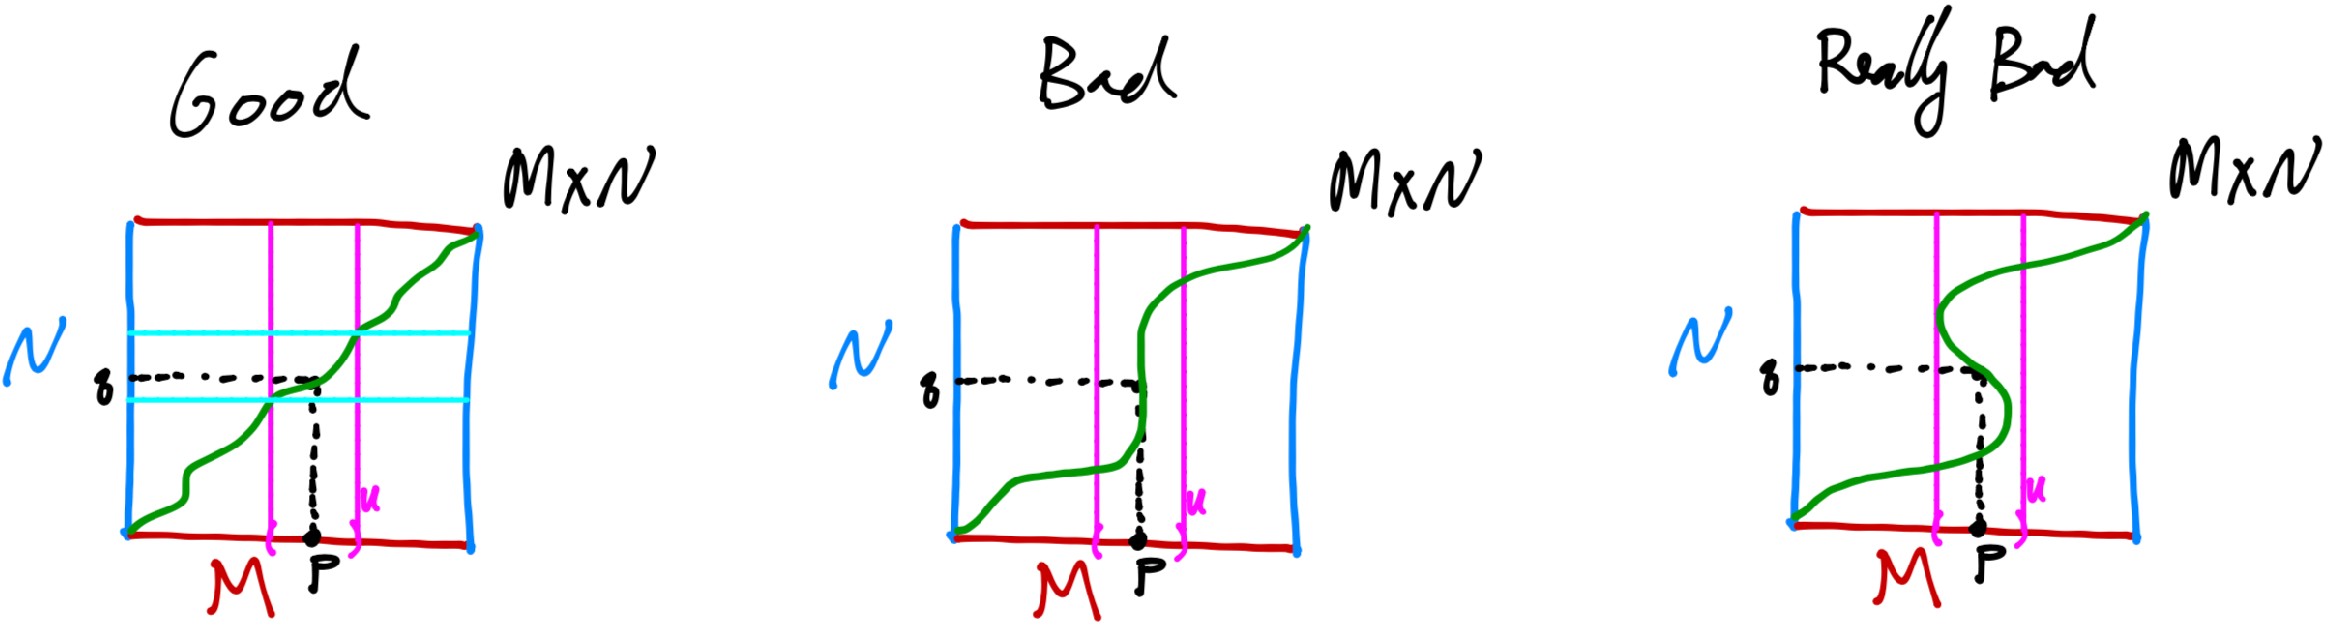
\includegraphics[height=1.3in]{badintegralmanifolds}
		\caption{Three possibilities for the integral submanifold $S$ of the ideal $\mathcal{I}$.}
		\alttext{Three depictions of the integral manifold $S$ inside $M \times N$. The product manifold $M \times N$ is depicted as a square, and $S$ is shown as a curve connecting the bottom-left and top-right corners of the square. In the first case, labeled ``Good,'', the curve is monotonically increasing. In the second, labeled ``Bad,'' it is still monotone but has a vertical tangency in the middle of the square. In the third, labeled ``Really Bad,'' it fails the vertical line test.}
		\label{fig:bad integral manifolds}
	\end{figure}
	
	In particular, I claim that $\left.d\pi_1 \right|_S$ is injective. To see this, let $(r,s) \in S$ and let $v \in T_{(r,s)} S$. If $d\pi_1(v) = 0$, then
	\begin{enumerate}
		\item $\mu_i(v) = 0$ for all $i=1, \dots , n$ since $\mathcal{I}$ consists of all the forms which vanish on the tangent space to $S$.
		\item $\pi_1^\ast \alpha_i(v) = \alpha_i(d\pi_1 v) = \alpha_i(0) = 0$.
	\end{enumerate}
	But then these two facts together imply that 
	\[
		\pi_2^\ast\omega_i(v) = \pi_1^\ast \alpha_i(v) - \mu_i(v) = 0-0=0
	\]
	for all $i=1, \dots , n$. Since the $\omega_i$ form a basis of 1-forms on $N$, this means that $d\pi_2(v) = 0$.
	
	In turn, this implies that $v = 0$ since $T_{(r,s)} M \times N = T_r M \oplus T_s N$. Since $(r,s) \in S$ was arbitrary, we see that $\left. d\pi_1 \right|_S$ is injective, so the Inverse Function Theorem (\Cref{thm:inverse function theorem}) implies that $\left. \pi_1 \right|_S \from S \to M$ is a local diffeomorphism since $\dim S = (m+n)-n=m=\dim M$. Therefore, there exists a neighborhood $V$ of $(p,q)$ in $S$ and a neighborhood $U$ of $p$ in $M$ so that $\left. \pi_1 \right|_V \from V \to U$ is a diffeomorphism.
	
	We're finally ready to define $f \from U \to N$ by $f = \pi_2 \circ \left(\left. \pi_1\right|_V\right)^{-1}$. Of course now we need to check that $f^\ast \omega_i = \alpha_i$ for all $i=1, \dots , n$. To see this, pick $i \in \{1, \dots , n\}$ and $u \in T_pM$. Then
	\begin{multline*}
		f^\ast \omega_i(u) = \left(\pi_2 \circ \left( \left. \pi_1 \right|_V\right)^{-1}\right)^\ast \omega_i(u) = \left(\left(\left. \pi_1\right|_V \right)^{-1}\right)^\ast \pi_2^\ast \omega_i(u) \\
		= \pi_2^\ast \omega_i\left(d\left(\left. \pi_1 \right|_V\right)^{-1} u \right) = \pi_1^\ast \alpha_i\left( d\left(\left. \pi_1 \right|_V\right)^{-1} u \right) - \mu_i \left(d\left(\left. \pi_1 \right|_V\right)^{-1} u  \right)
	\end{multline*}
	by the definition of $\mu_i = \pi_1^\ast \alpha_i - \pi_2^\ast \omega_i$. The second term above is zero since $d\left(\left. \pi_1 \right|_V\right)^{-1} u \in T_{(r,s)}S$ and $\mathcal{I} = \mathcal{I}(S)$ is generated by the $\mu_i$. Hence, we can continue the above computation to see
	\[
		f^\ast \omega_i(u) = \pi_1^\ast \alpha_i\left( d\left(\left. \pi_1 \right|_V\right)^{-1} u \right)  = \alpha_i \left(d \pi_1 d \left(\left. \pi_1 \right|_V\right)^{-1} u \right) = \alpha_i \left( d\left( \pi_1 \circ \left(\left. \pi_1 \right|_V\right)^{-1}\right)u\right) = \alpha_i(u)
	\]
	since $\pi_1 \circ \left(\left. \pi_1 \right|_V\right)^{-1}$ is just the identity map.
\end{proof}

\begin{exercise}
	Prove that the $f$ defined in the above proof is unique.
\end{exercise}

Now let's apply this result to proving \Cref{thm:identical Lie algebra homomorphisms imply identical Lie group homomorphisms}, which I restate for convenience:

\begin{theorem*}[\Cref{thm:identical Lie algebra homomorphisms imply identical Lie group homomorphisms}]
	Let $G$ be a connected Lie group and let $f_1, f_2 \from G \to H$ be Lie group homomorphisms so that the Lie algebra homomorphisms $df_1, df_2 \from \mathfrak{g} \to \mathfrak{h}$ are identical. Then $f_1 \equiv f_2$.
\end{theorem*}

\begin{proof}
	Since $df_1 = df_2$ as maps $ \mathfrak{g} \to \mathfrak{h}$, their dual maps $f_1^\ast = f_2^\ast$ as maps $\mathfrak{h}^\ast \to \mathfrak{g}^\ast$, where we identify $\mathfrak{g}^\ast$ and $\mathfrak{h}^\ast$ with the left-invariant 1-forms on $G$ and $H$, respectively.
	
	Suppose $\omega_1, \dots , \omega_n$ is a basis for the left-invariant 1-forms on $H$. Then we know that $f_1^\ast \omega_i = f_2^\ast \omega_i$ for all $i=1, \dots , n$. By uniqueness in \Cref{thm:map with specified forms}, it will follow that $f_1 \equiv f_2$ if we can show that the ideal $\mathfrak{I}$ on $G \times H$ generated by the
	\[
		\mu_i = \pi_1^\ast f_1^\ast \omega_i - \pi_2^\ast \omega_i
	\]
	is a differential ideal. It suffices to show that the $d\mu_i \in \mathcal{I}$, since a general element of $\mathcal{I}$ will be a linear combination of terms of the form $\beta_1 \wedge \dots \wedge \beta_\ell \wedge \mu_i \wedge \beta_{\ell+1} \wedge \dots \wedge \beta_k$, the exterior derivative of which will be a linear combination of wedge products which always include either $\mu_i$ or $d\mu_i$.
	
	So let's compute. First, notice that $\omega_1, \dots , \omega_n$ is a basis for the left-invariant forms on $H$, so $\left\{\omega_i \wedge \omega_j : i < j \right\}$ is a basis for the left-invariant 2-forms on $H$. Since $d\omega_k$ is left-invariant for any $k \in \{1, \dots, n\}$, there exist constants $c_{ij}^k$ so that
	\[
		d\omega_k = \sum_{i < j} c_{ij}^k \omega_i \wedge \omega_j.
	\]
	But then
	\begin{align*}
		d\mu_k & = d\left(\pi_1^\ast f_1^\ast \omega_k - \pi_2^\ast \omega_k\right) \\
		& = \pi_1^\ast f_1^\ast d\omega_k - \pi_2^\ast d\omega_k \\
		& = \pi_1^\ast f_1^\ast \sum_{i < j} c_{ij}^k \omega_i \wedge \omega_j - \pi_2^\ast \sum_{i < j} c_{ij}^k \omega_i \wedge \omega_j \\
		& = \sum_{i<j} c_{ij}^k \left( \pi_1^\ast f_1^\ast \omega_i \wedge \pi_1^\ast f_1^\ast \omega_j - \pi_2^\ast \omega_i \wedge \pi_2^\ast\omega_j\right) \\
		& =  \sum_{i<j} c_{ij}^k \left( \left(\pi_1^\ast f_1^\ast \omega_i -\pi_2^\ast \omega_i \right)\wedge \pi_1^\ast f_1^\ast \omega_j + \pi_2^\ast \omega_i \wedge \left(\pi_1^\ast f_1^\ast \omega_j - \pi_2^\ast \omega_j \right)\right) \\
		& =  \sum_{i<j} c_{ij}^k \left( \mu_i\wedge \pi_1^\ast f_1^\ast \omega_j + \pi_2^\ast \omega_i \wedge \mu_j\right) 
	\end{align*}
	by adding and subtracting a term of the form $\pi_2^\ast \omega_i \wedge \pi_1^\ast f^\ast \omega_j$ in going from the fourth to the fifth line. But then each $ \mu_i\wedge \pi_1^\ast f_1^\ast \omega_j + \pi_2^\ast \omega_i \wedge \mu_j \in \mathcal{I}$, so we conclude that $d\mu_k \in \mathcal{I}$, and hence $\mathcal{I}$ is a differential ideal.
\end{proof}

With all of this done, we have now proved uniqueness in \Cref{thm:Lie group Lie algebra correspondence}, which I restate:

\begin{theorem*}[\Cref{thm:Lie group Lie algebra correspondence}]
	Let $G$ and $H$ be Lie groups with Lie algebras $\mathfrak{g}$ and $\mathfrak{h}$, respectively, and with $G$ simply-connected. Let $\psi \from \mathfrak{g} \to \mathfrak{h}$ be a Lie algebra homomorphism. Then there exists a unique Lie group homomorphism $\phi \from G \to H$ so that $d\phi = \psi$.
\end{theorem*}

I also restate \Cref{cor:sc Lie groups determined by Lie algebra}, which follows immediately:
\begin{corollary*}[\Cref{cor:sc Lie groups determined by Lie algebra}]
	If $G$ and $H$ are simply-connected and have isomorphic Lie algebras, then $G \cong H$.
\end{corollary*}

Since we have proved uniqueness in \Cref{thm:Lie group Lie algebra correspondence}, it remains to show existence, which we do by defining $\phi \from G \to H$ as in the proof of \Cref{thm:map with specified forms} by $\phi = \pi_2 \circ \left(\left. \pi_1\right|_S\right)^{-1}$ with $S \subset G \times H$ with $\mathcal{I} = \mathcal{I}(S)$. The key point is that the definition of the $\mu_i = \pi_1^\ast \psi^\ast \omega_i - \pi_2^\ast \omega_i$ which generate $\mathcal{I}$ depends only on $\psi \from \mathfrak{g} \to \mathfrak{h}$ and not on the $\phi$ that needs to be constructed. Proving that $\phi$ is really a homomorphism depends on some covering space theory that I don't really want to get into, but suffice it to say that this is true.

Notice that the simply-connected hypothesis in \Cref{cor:sc Lie groups determined by Lie algebra} is essential, since $\orthog(n)$ and $\SO(n)$ have identical Lie algebras even though they're not isomorphic as Lie groups (nor even homeomorphic). Admittedly, this feels like a cheat since it's really only using connectedness, and of course $\orthog(n)$ and $\SO(n)$ do have the same connected component of the identity, which is all that the Lie algebra could plausibly detect.

But we've already seen a less trivial example in \Cref{prop:accidental isomorphisms}, which showed that $\mathfrak{so}(3) \cong \mathfrak{su}(2)$, yet $\SO(3)$ and $\SU(2)$ are not isomorphic as groups (nor even homeomorphic as topological spaces). It is fairly easy to see that these groups are not isomorphic since they have different centers:
\[
	Z(\SO(3)) = \{I\}, \quad \text{but} \quad Z(\SU(2)) = \{I, -I\} \cong \Z/2\Z.
\]

In fact, as topological spaces $\SO(3) \cong \RP^3$ and $\SU(2) \cong S^3$, so these spaces have different fundamental groups: $\pi_1\left(\RP^3\right) \cong \Z/2\Z$ and $\pi_1\left(S^3\right) = \{1\}$. Hence, they cannot be homeomorphic either. Looked at this way, $S^3$ is the universal cover of $\RP^3$, meaning that $\SU(2)$ is homeomorphic to the universal cover of $\SO(3)$, and hence also to $\operatorname{Spin}(3)$.\footnote{In general, $\Spin(n)$ is the universal cover of $\SO(n)$.}